\section{Definition}
Um einen Zero-Knowledge-Beweis definieren zu können, muss man sich erst einmal auf eine konkrete Definition eines Beweises festlegen. Im allgemeinen mathematischen Ver\-ständ\-nis ist dieser eine von einem Beweiser aufgeschriebene statische Zeichenkette \( \pi \), in dem eine Aussage mithilfe von Axiomen und Schlussregeln so hergeleitet wird, dass jeder Verifizierer sich selbst von der Korrektheit der Aussage überzeugen kann.

\cite{goldwasser1989} verallgemeinert den Beweisbegriff: Zum einen wird Interaktion zugelassen, das heißt, der Verifzierer \( V \) kann dem Beweiser \( P \) Fragen stellen, auf die jener antworten kann. Außerdem muss der Verifizierer nicht mit letzter Sicherheit überzeugt sein, es genügt, wenn dieser mit einer sehr hohen Sicherheit (von beispielsweise \( 99,9  \% \)) von der Aussage überzeugt werden kann.\footnote{vgl. \cite[Seite 2]{princeton}}
 
\subsection{Interaktive Protokolle}

Wie kann man aber so ein Beweissystem formal fassen? Hierzu werden die einzelnen Teilnehmer als eine Erweiterung einer normalen Turing-Maschine festgelegt. Das Alphabet der Sprachen (hier bezeichnet mit  dem Symbol \( L \)) sei in der gesamten Arbeit \( \Sigma = \left\lbrace 0, 1 \right\rbrace \).

% TODO: Abstand
\vspace{0.2cm}

\begin{definition}[Interaktive Turing-Maschine]
Eine Interaktive Turing Maschine (kurz ITM) ist eine Sechs-Band-Turing-Maschine mit einem \textnormal{Arbeitsband}, einem nur-lesbaren \glqq{}öffentlichen\grqq{} \textnormal{Eingabeband},einem nur-lesbaren \glqq{}privaten\grqq{} Eingabeband, jeweils einem nur-les- bzw. nur-beschreibbaren \textnormal{Kommunikationsband} und einem \textnormal{Zufallszahlenband}, das mit Zufallsbits beschrieben ist.\footnote{vgl. \cite[Definition 1.1]{np}, \cite[Abschnitt 2.1]{goldwasser1989} und geheimes Eingabeband aus \cite[Chapter 2]{identity}}
\end{definition}

Zwei solcher Automaten gemeinsam können dann ein Protokoll beschreiben:

% TODO: Abstand
\vspace{0.2cm}

\begin{definition}[Interaktives Protokoll]
Ein interaktives Protokoll ist ein geordnetes Paar \( \left< P, V \right> \) zweier ITMs, die sich das \glqq{}öffentliche\grqq{} Eingabeband teilen und jeweils das beschreibbare Kommunikationsband der einen das lesbare Kommunikationsband der anderen ITM ist. Beide Maschinen führen ihre Berechnung abwechselnd durch: Während die eine rechnet, befindet sich die andere im \glqq{}Leerlauf\grqq{}. Das Wort, das von einer während eines einzelnen Berechnungsschrittes auf das Band geschrieben wird, wird als die zur anderen ITM \textnormal{gesendete Nachricht} bezeichnet.\footnote{vgl. \cite[Abschnitt 2.1]{goldwasser1989} und \cite[Definition 1.3]{np}}
\end{definition}

Die beiden interaktiven Turing-Maschinen \( \left< P, V\right> \) sind hier das Modell für den Beweiser \( P \) und den Verifizierer \( V \). Eine Kommunikation der beiden probabilistischen Maschinen mit der gemeinsamen Eingabe \( \omega \) kann auch als Zufallsvariable \( \left< P, V \right> \left( \omega \right) \) aufgefasst werden.

\vspace{1em}
\begin{minipage}{\linewidth}
	\centering
	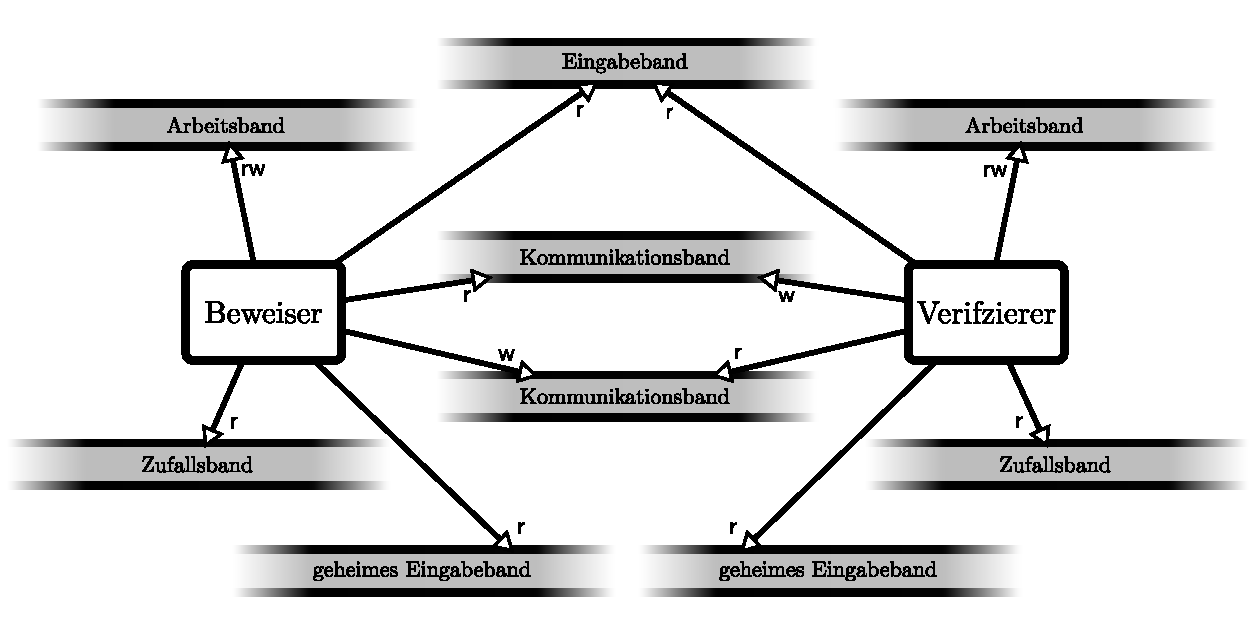
\includegraphics[width=0.9\linewidth]{img/interactiveprotocol.pdf}
	\captionof{figure}[Interaktives Protokoll]{Interaktives Protokoll mit Beweiser \( P \) und Verifizierer \( V \)}
	\label{fig:interactiveprotocol}
\end{minipage}

% TODO: Abstand
\vspace{0.2cm}

\begin{definition}[Interaktive Beweissysteme]
\label{definition:proofsystem}
Ein interaktives Beweissystem ist ein interaktives Protokoll 
\( \left< P, V\right> \). Dabei ist die Laufzeit von \( V \) und \( P \) polynomiell bezüglich des Wortes auf dem Eingabeband beschränkt. Das geheime Eingabeband des Beweisers beinhaltet die Lösung des Problems, das des Verifizierers bleibt leer. Zusätzlich sei erfüllt:\footnote{In den meisten Werken zu dem Thema (wie z.B. \cite{np}) kann der Beweiser eine unbegrenzte Laufzeit besitzen und hat dafür kein geheimes Eingabeband. Da in keinem der hier besprochenen Beispielen dies benötigt wird, habe ich mich stattdessen für eine polynomielle Laufzeit und ein geheimes Eingabeband entschieden. Siehe \cite[Chapter 2]{identity}, \cite[Definition 1]{20yearszeroknowledge} und \cite[Definition 2]{np}}
\begin{itemize}

\item[\textnormal{Vollständigkeit:}] \( \forall \omega \in L : \textnormal{\textbf{\textsf{P}}} \left( V \textnormal{ akzeptiert bei } \left< P, V \right> \left( \omega \right) \right) = 1 \)  \glqq{}Für jedes \( \omega \in L \) akzeptiert \( V \) immer nach der Durchführung des Beweises mit dem Beweiser \( P \).\grqq{}

\item[\textnormal{Korrektheit:}] \( \exists p \textnormal{ Polynom}: \forall \omega \notin L, P^{\ast} \textnormal{ beliebige ITM} : \textnormal{\textbf{\textsf{P}}} \left( V \textnormal{ akzeptiert bei } \left< P ^{\ast}, V \right> \left( \omega \right) \right) \leq \frac{1}{p \left( \left| \omega \right| \right)}  \) \glqq{}Für jedes \( \omega \notin L \) gibt es keine Strategie, mit der der Verfizierer \glqq{}immer\grqq{} überzeugt werden kann.\grqq{}
\end{itemize}
\end{definition}

 Falls \( V \) akzeptiert (also überzeugt werden konnte) oder verwirft, vermerkt er dies auf seinem Kommunikationsband und beendet das Protokoll.

\subsection{Zero Knowledge}
Informell bedeutet Zero Knowledge, dass egal, was der Verifizierer versucht, er keine zusätzlichen Informationen aus dem Beweiser bekommen kann, die er sich mit seiner polynomiellen Beschränkung nicht hätte selbst berechnen können. Dies wird hier durch einen ebenfalls im Erwartungswert polynomiellen Simulator definiert, der den Verfizierer bekommt und anhand dessen eine mögliche Kommunikation zwischen diesem Verifizierer und dem im Protokoll spezifizierten Beweiser ausgibt, welche für einen polynomiellen Algorithmus ununterscheidbar von einer echten Kommunikation ist. Dabei soll es egal sein, ob der Verifizierer \textit{ehrlich} ist, sich also an das Protokoll hält, oder ob er bewusst versucht, durch falsche Eingaben den Beweiser zu für ihn nützlichen Aussagen zu bringen.

Was hier noch für die vollständige Definition von Ze ro Knowledge fehlt, ist eine Möglichkeit auszusagen, dass sich zwei verschiedene Zufallsvariablen genug ähneln, sodass diese für eine polynomiell beschränkte Turing-Maschine nicht unterscheidbar sind.

% TODO: Abstand
\vspace{0.2cm}

\begin{definition}[Rechnerische Ununterscheidbarkeit] Sei \( L \) eine Sprache.
Zwei in der Länge polynomiell beschränkte Zufallsvariablen \( U \left( \omega \right) \) und \( V \left( \omega \right) \) über \( L \) sind rechnerisch ununterscheidbar, falls für jeden im Erwartungswert polynomiellen Algorithmus \( C \) und für jedes Polynom \( p \) bei ausreichend langem \( \omega \in L \) gilt:\footnote{vgl. \cite[Seite 93]{goldwasser1989}}
\[ \left| \textnormal{\textbf{\textsf{P}}} \left( C \left( U \left( \omega \right) \right) = 1 \right) - \textnormal{\textbf{\textsf{P}}} \left( C \left( V \left( \omega \right) \right) = 1 \right) \right| < \frac{1}{p \left( \left| \omega \right| \right)} \]
\end{definition}

Da man das Ergebnis nicht-deterministischer Berechnungen als Zufallsvariable auffassen kann, lässt sich nun Zero Knowledge definieren:

% TODO: Abstand
\vspace{0.2cm}

\begin{definition}[Zero Knowledge]
\label{definition:zeroknowledge}
Ein Beweiser \( P \) ist genau dann (rechnerisch) \textnormal{Zero Knowledge} auf Eingabewörtern aus \( L \), wenn für jeden probabilistisch-polynomiellen Verifizierer \( V ^ {\ast} \) eine im Erwartungswert polynomielle Turing-Maschine \( M_{V^{\ast}} \) existiert, die die Kommunikation zwischen \( P \) und \( V^{\ast} \) simuliert, sodass folgende Familien von Zufallsvariablen rechnerisch ununterscheidbar sind:\footnote{vgl. \cite[Definition 4]{20yearszeroknowledge}}
\begin{enumerate}
\item[1.] \( \left\lbrace \left< P, V^{\ast} \right> \left( \omega \right) \right\rbrace _{\omega \in L} \) \( \overset{\textnormal{def}}{=} \) die Kommunikation zwischen \( V ^ {\ast}\) und \( P \) bei gemeinsamer Eingabe \( \omega \in L \).
\item[2.] \( \left\lbrace M_{V^{\ast}} \left( \omega \right) \right\rbrace _{\omega \in L} \) \( \overset{\textnormal{def}}{=} \) die Ausgabe des Simulators \( M_{V^{\ast}} \) bei der Eingabe von \( \omega \in L \). 
\end{enumerate}
\end{definition}

\pagebreak
